\part{Agents}
\frame{\partpage}

\begin{frame}{Agents}
    \begin{center}
        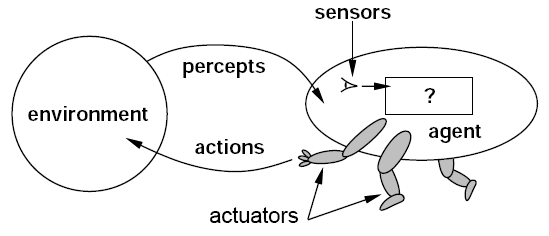
\includegraphics[width=0.7\textwidth]{agent}

        \vspace{2ex}

        \pause An \textbf{agent} is anything which perceives an \textbf{environment} through \textbf{sensors},
            and acts upon that environment through \textbf{actuators}.
    \end{center}
\end{frame}

\begin{frame}{Performance}
    \begin{itemize}
        \pause\item An ``intelligent'' agent moves towards some kind of \textbf{goal}
        \pause\item The goal is an \textbf{environment state} (or a set of states)
        \pause\item A \textbf{performance measure} evaluates a given state for how well it fits the goal
    \end{itemize}
\end{frame}

\begin{frame}{PEAS}
    For each example of an agent, what are the \underline{P}erformance measure,
        \underline{E}nvironment, \underline{A}ctuators and \underline{S}ensors?
    
    \begin{itemize}
        \pause\item A Roomba
        \pause\item A self-driving car
        \pause\item A chatbot
        \pause\item A factory robot
        \pause\item An enemy in an FPS game
        \pause\item A chess AI
        \pause\item A human
    \end{itemize}
\end{frame}

\begin{frame}{Types of environment}
    \begin{itemize}
        \pause\item Environments come with many different properties
        \pause\item These properties influence the choice of AI architecture we use to build agents
    \end{itemize}
\end{frame}

\begin{frame}{Observability}
    \begin{itemize}
        \pause\item \textbf{Fully observable}: the agent's sensors give it full information about the state of the environment
        \pause\item \textbf{Partially observable}: some aspects of the environment state are not visible to the agent's sensors
        \pause\item E.g.\ a chess game is fully observable, a poker game is partially observable
    \end{itemize}
\end{frame}

\begin{frame}{Number of agents}
    \begin{itemize}
        \pause\item \textbf{Single agent}: our agent is the only one in the environment
        \pause\item \textbf{Multi-agent}: there is more than one agent
        \pause\item \textbf{Cooperative}: all agents share the same performance measure
        \pause\item \textbf{Competitive}: agents' performance measures are in opposition to each other
            (i.e.\ if one agent ``wins'', another ``loses'')
    \end{itemize}
\end{frame}

\begin{frame}{Determinism}
    \begin{itemize}
        \pause\item \textbf{Deterministic}: the next state of the environment is completely determined by the current state and by the agent's action
        \pause\item \textbf{Stochastic}: there is some aspect of randomness in determining the next state
        \pause\item E.g.\ chess is deterministic; any board game involving dice rolls or random card draws is stochastic
    \end{itemize}
\end{frame}

\begin{frame}{Dynamicity}
    \begin{itemize}
        \pause\item \textbf{Static}: the environment does not change while the agent is deliberating
        \pause\item \textbf{Dynamic}: the environment changes constantly
        \pause\item E.g.\ most board games are static, most (non turn-based) video games are dynamic
    \end{itemize}
\end{frame}

\begin{frame}{Discreteness}
    \begin{itemize}
        \pause\item \textbf{Discrete}: time, percepts and actions are all discrete
            (from a finite set of possibilities or ``integer valued'')
        \pause\item \textbf{Continuous}: at least one of these is not discrete
            (``float valued'')
        \pause\item Continuous problems are hard so we sometimes \textbf{discretise} them
    \end{itemize}
\end{frame}

\begin{frame}{Known or unknown}
    \begin{itemize}
        \pause\item Are all the details of the environment \textbf{known} to the AI designer?
        \pause\item For a game or simulation: probably \textbf{yes}
            (unless someone else made it and we don't have the source code)
        \pause\item For the real world: technically \textbf{no}
            (but we have physics, sociology, economics etc to give us good approximations)
    \end{itemize}
\end{frame}

\begin{frame}{Agents and AI}
    \begin{itemize}
        \pause\item The ideas of agents and environments are a useful frame for designing AI
        \pause\item All(?) AI problems can be expressed in terms of creating an agent
            that optimises some performance measure in some environment
        \pause\item Agent design boils down to: given a \textbf{percept} (and possibly some \textbf{memory} of past percepts/actions),
            choose the best \textbf{action} to take now
    \end{itemize}
\end{frame}
